% ===================================================================
% FILE: Lezione6.tex
% ===================================================================

\part{Lezione 22 (10/11/2025) }

\section{Mergesort }
Mergesort è un algoritmo di ordinamento basato su Divide et Impera .
\begin{definition}[Mergesort: Paradigma D\&I]
\begin{itemize}
    \item \textbf{DIVIDE} : Divide l'array $A[p..r]$ in due metà, $A[p..q]$ e $A[q+1..r]$, dove $q = \lfloor (p+r)/2 \rfloor$ .
    \item \textbf{IMPERA} : Ordina ricorsivamente le due metà chiamando `Mergesort(A, p, q)` e `Mergesort(A, q+1, r)` .
    \item \textbf{COMBINE} : Combina (fonde) i due sottoarray ordinati $A[p..q]$ e $A[q+1..r]$ in un unico array ordinato $A[p..r]$ tramite la procedura `Merge(A, p, q, r)` .
\end{itemize}
\end{definition}

\subsection{Pseudocodice Mergesort}
\begin{algorithmic}[1]
\Procedure{Mergesort}{A, p, r} 
    \If{$p < r$} 
        \State $q = \lfloor (p+r)/2 \rfloor$ \Comment{DIVIDE }
        \State \Call{Mergesort}{A, p, q} \Comment{IMPERA }
        \State \Call{Mergesort}{A, q+1, r} \Comment{IMPERA }
        \State \Call{Merge}{A, p, q, r} \Comment{COMBINE }
    \EndIf
\EndProcedure
\end{algorithmic}

\subsection{Procedura Merge }

\begin{observation}[Procedura Merge]
La procedura `Merge` fonde due sottoarray contigui $A[p..q]$ e $A[q+1..r]$, che si assumono \textbf{già ordinati}.
Ha complessità \textbf{Lineare} $T(n) = \Theta(n)$ , dove $n = r-p+1$ .
Utilizza due array di appoggio, $L$ e $R$ , e due "sentinelle" ($\infty$) per evitare controlli sull'indice .
\end{observation}

\begin{algorithmic}[1]
\Procedure{Merge}{A, p, q, r} 
    \State $n_1 = q - p + 1$ \Comment{Dim. primo sottoarray }
    \State $n_2 = r - q$ \Comment{Dim. secondo sottoarray }
    \State Crea array $L[1..n_1+1]$ e $R[1..n_2+1]$ 
    
    \Comment{Copia i dati negli array di appoggio}
    \For{$i = 1 \to n_1$}
        \State $L[i] = A[p + i - 1]$ 
    \EndFor
    \For{$j = 1 \to n_2$}
        \State $R[j] = A[q + j]$ 
    \EndFor
    
    \State $L[n_1 + 1] = +\infty$ \Comment{Sentinella }
    \State $R[n_2 + 1] = +\infty$ \Comment{Sentinella }
    
    \State $i = 1$ \Comment{Indice per $L$ }
    \State $j = 1$ \Comment{Indice per $R$ }
    
    \Comment{Fondi L e R nell'array A}
    \For{$k = p \to r$} 
        \If{$L[i] \le R[j]$} 
            \State $A[k] = L[i]$ 
            \State $i = i + 1$ 
        \Else
            \State $A[k] = R[j]$
            \State $j = j + 1$
        \EndIf
    \EndFor
\EndProcedure
\end{algorithmic}

\subsection{Analisi Complessità Mergesort }

\begin{definition}[Analisi Mergesort: Ricorrenza]
\textbf{Equazione di Ricorrenza:}
$a=2$ sottoproblemi, $n/b = n/2$.
$f(n) = D(n) \text{ (cost.)} + C(n) \text{ (Merge)} = \Theta(1) + \Theta(n) = \Theta(n)$.
$$ T(n) = \begin{cases} \Theta(1) & \text{se } n = 1 \text{ } \\ 2T(n/2) + \Theta(n) & \text{se } n > 1 \text{ } \end{cases} $$
\end{definition}

\textbf{Soluzione 1: Albero di Ricorsione} 
L'albero di ricorsione mostra il costo $f(n_i)$ ad ogni livello.
\begin{center}
\begin{tikzpicture}[
    level distance=1.5cm, 
    level 1/.style={sibling distance=5cm},
    level 2/.style={sibling distance=2.5cm},
    level 3/.style={sibling distance=1.2cm},
    level 4/.style={sibling distance=0.8cm},
    every node/.style={draw, circle, inner sep=1pt, minimum size=6mm, font=\small},
    ]
  % Albero
  \node (z){$n$}
    child {node {$n/2$} 
      child {node {$n/4$} 
        child {node[draw=none] {$\vdots$}
            child{node {$1$} }
        }
      } 
      child {node {$n/4$}
        child {node[draw=none] {$\vdots$}
            child{node {$1$}}
        }
      }
    }
    child {node {$n/2$} 
      child {node {$n/4$} 
         child {node[draw=none] {$\vdots$}
            child{node {$1$}}
         }
      } 
      child {node {$n/4$}
         child {node[draw=none] {$\vdots$}
            child{node {$1$}}
         }
      }
    };
  % Costi
    \node[right=of z, xshift=5cm, draw=none, font=\small] (l0) {Costo: $cn$ };
    \node[right=of z, xshift=5cm, yshift=-1.5cm, draw=none, font=\small] (l1) {Costo: $2 \cdot c(n/2) = cn$ };
    \node[right=of z, xshift=5cm, yshift=-3cm, draw=none, font=\small] (l2) {Costo: $4 \cdot c(n/4) = cn$ };
    \node[right=of z, xshift=5cm, yshift=-4.5cm, draw=none, font=\small] (l3) {$\vdots$};
    \node[right=of z, xshift=5cm, yshift=-6cm, draw=none, font=\small] (l4) {Costo (foglie): $n \cdot c(1) = \Theta(n)$ };
  % Altezza
    \draw[decorate, decoration={brace, amplitude=10pt}] (l0.north west) ++ (-12, 0.5) -- (l4.south west) ++ (-12, -0.5) node [midway, left, xshift=-10pt, font=\small] {Altezza $\log_2 n$};
    \node[below=of l4, yshift=-1cm, draw=none, font=\small] {Totale: $\sum_{i=0}^{\log_2 n - 1} cn + \Theta(n) = cn \log_2 n + \Theta(n) = \Theta(n \log n)$};
\end{tikzpicture}
\end{center}
Il costo per ogni livello è $cn$ . L'albero ha $\log_2 n$ livelli.
Il costo totale è $cn \cdot \log_2 n = \Theta(n \log n)$ .
\begin{observation}[Analisi Mergesort: Metodo Iterativo]
\textbf{Soluzione 2: Metodo Iterativo (Sostituzione)} 
$T(n) = 2T(n/2) + cn$ 
$T(n) = 2(2T(n/4) + c(n/2)) + cn = 4T(n/4) + cn + cn = 4T(n/4) + 2cn$ 
$T(n) = 4(2T(n/8) + c(n/4)) + 2cn = 8T(n/8) + cn + 2cn = 8T(n/8) + 3cn$ 
... dopo $i$ passi ...
$T(n) = 2^i T(n/2^i) + i \cdot cn$ 
Ci si ferma al caso base $n/2^i = 1 \implies i = \log_2 n$.
$T(n) = 2^{\log_2 n} T(1) + (\log_2 n) \cdot cn$ 
$T(n) = n \cdot \Theta(1) + cn \log_2 n = \Theta(n \log n)$ .
\end{observation}


\begin{observation}[Complessità in Spazio: Mergesort]
Mergesort \textbf{non} ordina "in loco" , poiché richiede $\Theta(n)$ spazio ausiliario per gli array $L$ e $R$ ad ogni chiamata di `Merge` .
\end{observation}

\subsection{Esempio: Albero delle Chiamate }
Per $A[1..7]$ , l'ordine delle chiamate ricorsive è :
\begin{center}
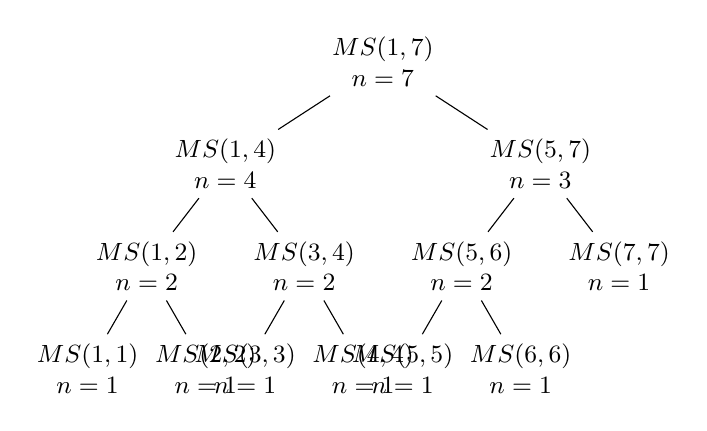
\begin{tikzpicture}[
    level distance=1.3cm,
    level 1/.style={sibling distance=4cm},
    level 2/.style={sibling distance=2cm},
    level 3/.style={sibling distance=1.5cm},
    every node/.style={align=center, font=\small}
    ]
  \node {$MS(1,7)$ \\ $n=7$ }
    child {node {$MS(1,4)$ \\ $n=4$ }
      child {node {$MS(1,2)$ \\ $n=2$ }
        child {node {$MS(1,1)$ \\ $n=1$ }}
        child {node {$MS(2,2)$ \\ $n=1$ }}
      } 
      child {node {$MS(3,4)$ \\ $n=2$ }
        child {node {$MS(3,3)$ \\ $n=1$ }}
        child {node {$MS(4,4)$ \\ $n=1$ }}
      }
    }
    child {node {$MS(5,7)$ \\ $n=3$ }
      child {node {$MS(5,6)$ \\ $n=2$ }
        child {node {$MS(5,5)$ \\ $n=1$ }}
        child {node {$MS(6,6)$ \\ $n=1$ }}
      } 
      child {node {$MS(7,7)$ \\ $n=1$ }}
    };
\end{tikzpicture}
\end{center}

\newpage